\documentclass[11pt,letterpaper]{article}
\usepackage[margin=1.0in]{geometry}
\usepackage[utf8]{inputenc}
\usepackage{cite}
\usepackage{amsmath}
\usepackage{amsfonts}
\usepackage{amssymb}
\usepackage{makeidx}
\usepackage{graphicx}
\usepackage{hyperref}
\setlength\parindent{0pt}

\author{STUDENT NAME}
\title{HW: RMS value of a triangular signal.}

\begin{document}

\maketitle

\begin{figure}
\centering
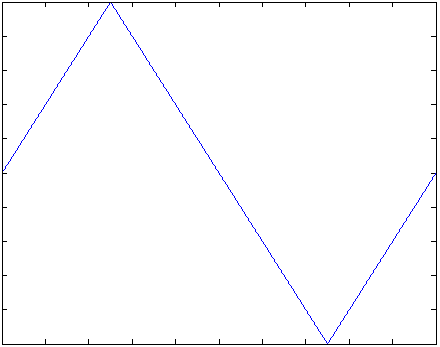
\includegraphics[width=0.8\linewidth]{TriangularWaveSignal}
\caption{Shown is a triangular signal without offset. The period of the signal is $T$, and you have to calculate the amplitude yourself. The functional form of the signal is $U(t) = at$ on the interval $[0, \dfrac{T}{4}]$. Annotating this graph with the given symbols is recommended.}
\label{fig:TriangularWaveSignal}
\end{figure}

Given is a triangular wave form as shown in Figure \ref{fig:TriangularWaveSignal}. Your job is to find out the ratio between the RMS value of any triangular wave form and its amplitude or $\dfrac{U_{RMS}}{U}$. The only thing you have to assume is that the signal is proportional to time as in $U(t) = at$ where $a$ is a constant. Then you have to calculate the RMS value using:

\begin{equation} \label{Eqn:ICE_RMS_Triangle_KEY1}
U_{RMS}^2=\dfrac{1}{T}\int_{t=0}^{t=T} U(t)^2 dt
\end{equation}

and divide by the Amplitude (which you also have to calculate). Hint: When you calculate the integral be smart about it, there is a lot of  symmetry in the signal, use that to your advantage.\\

You need to show ALL your steps and write them in LaTex functionality (copy over the equation given above and tweak it to your needs).\\

\textbf{Solution}\\



\end{document}
